\chapter{Literature Review}
\label{chap:lit.review}

\section{Introduction}

\subsection{Recurrent Neural Networks}

Recurrent Neural Networks (RNNs) are in forefront of recent development and advances in \textit{deep learning} by making able neural networks to deal with sequences data, which is a major shortcoming in ANN. If the data is based on sequence of events in a video or text, the traditional neural network can't do reasoning for a single event based on its previous one. To tackle this issue RNNs have loops which enables them to persist the information.

\begin{figure}[p]
	\centering
	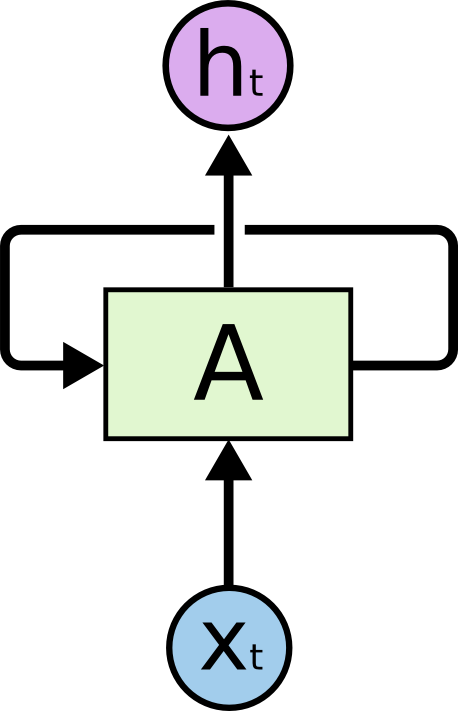
\includegraphics[scale=0.4]{./figs/rnn-rolled}
	\caption[A Rolled Recurrent Neural Networks]{Recurrent Neural Networks (RNNs) uses loops.}
	\label{fig:rnn-rolled}
\end{figure}

As it shown in \textbf{Figure \ref{fig:rnn-rolled}}, a selected neural network, $A$ takes the input $x_t$ and outputs the value of $h_t$. this might not show how data goes from one step to the next one in a same network until you unroll the loop and see chain architecture of recurrent neural networks that makes them the best choice for sequential data, \textbf{Figure \ref{fig:rnn-unrolled}}.

\begin{figure}[p]
	\centering
	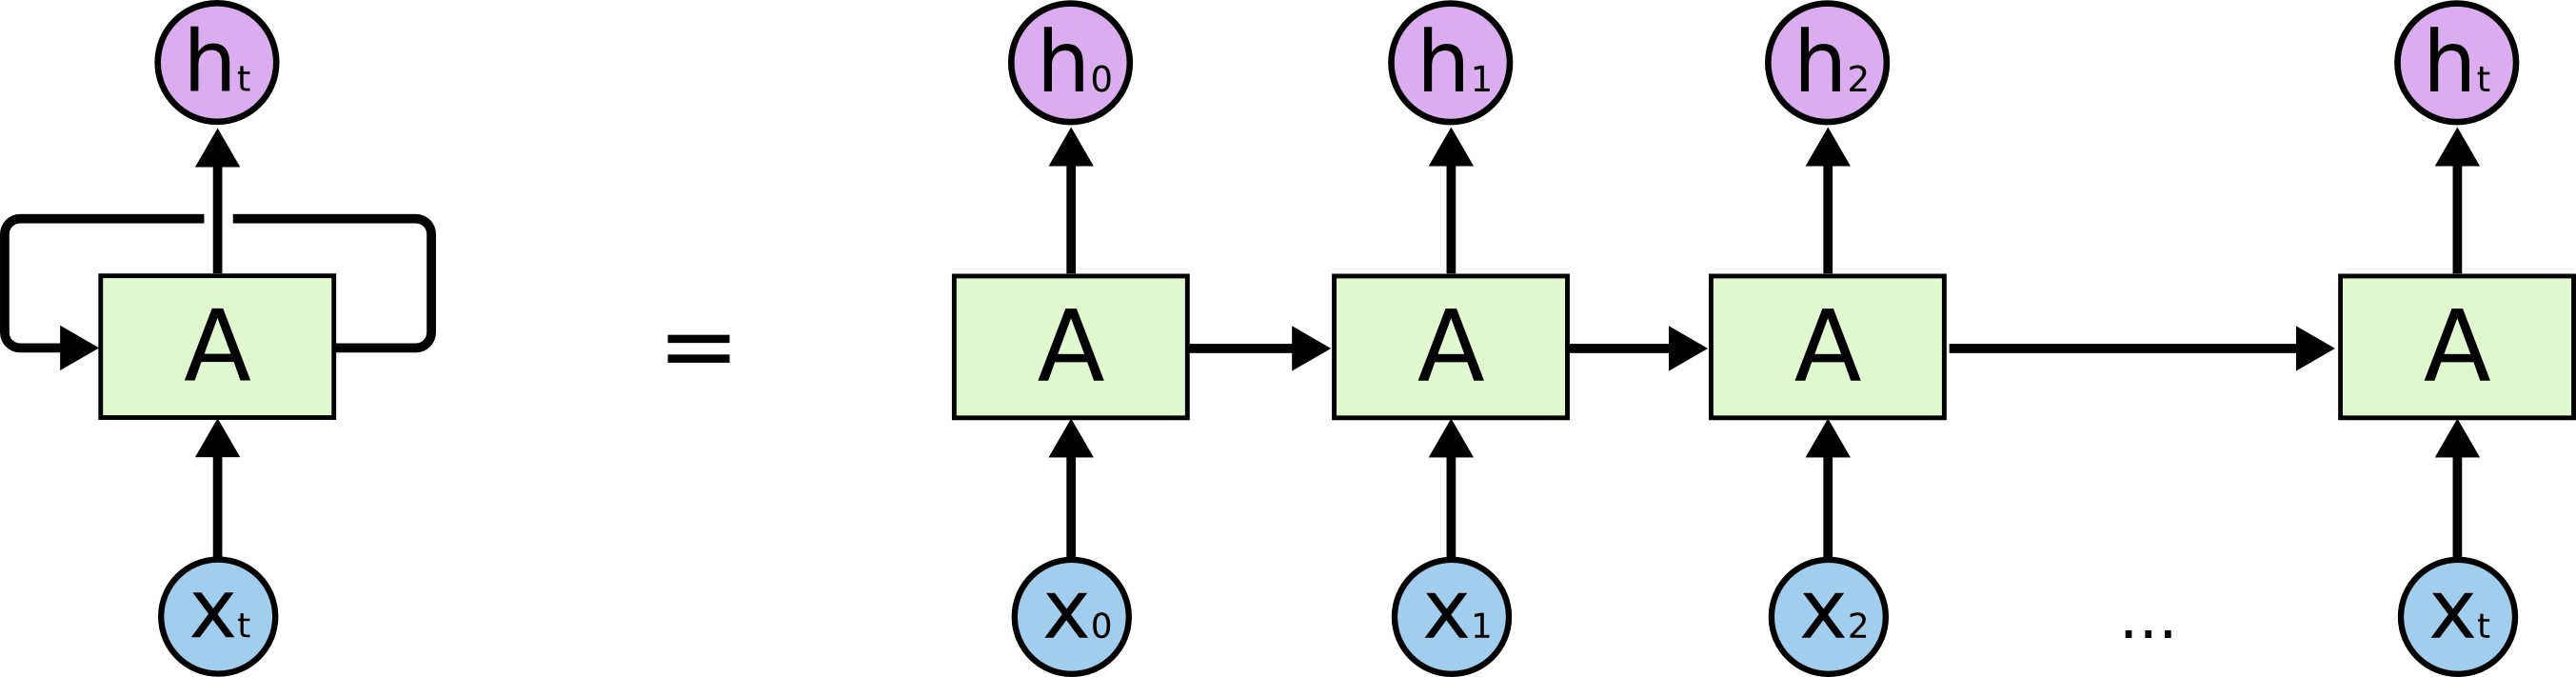
\includegraphics[scale=0.4]{./figs/rnn-unrolled}
	\caption[An Unrolled Recurrent Neural Networks]{An Unrolled Recurrent Neural Networks (RNNs).}
	\label{fig:rnn-unrolled}
\end{figure}

While RNNs is being used in variety of applications from language modeling to image captioning, the essential to all these achievement is the RNN-LSTMs \cite{Hochreiter1997}. An enhanced version of RNNs that outperforms better than the standard RNN.

\section{Similar Works}
Sharpening the posterior as proposed in Chapter \ref{chap:method} has mutualities with other techniques. Such as line search, where $\eta$ is a trained parameter that does line search along the gradient direction to give probabilistic interpretations to line search. In this work the novel technique is to use a variational posterior with the reparametrization gradient.

Another similar technique is dynamic evaluation \cite{Mikolov2010}, which trains the RNN during evaluation steps of the model with a fixed learning rate. The drawback of this technique is that each update applied in this case is cumulative, and only uses previously seen data.

Finally, learning to optimise \cite{Li2016a} is considered as similar work also since it is learned so supposedly it produces better updates than the rest suggested by AdaGrad \cite{Duchi2011} or Adam \cite{Kingma2013a}. Whilst they train a parametric model, we treat these as free parameters (so that they can adapt more quickly to the non-stationary distribution w.r.t. parameters). Notably, we use gradient information to inform a variational posterior so as to reduce variance of Bayesian Neural Networks. Thus, although similar in flavour, the underlying motivations are quite different.

\section{State-of-the-Arts}
Applying Bayesian methods to neural networks has a long history, with most common approximations having been tried.
\cite{buntine1991bayesian} propose various maximum a posteriori schemes for neural networks, including an approximate posterior
centered at the mode.
\cite{buntine1991bayesian} also suggest using second order derivatives in the prior to encourage smoothness of the resulting network.
\cite{Hinton1993} proposed using variational methods for compressing the weights of neural networks as a regulariser.
\cite{Hochreiter1995} suggest an MDL loss for single layer networks that penalises non-robust weights by means of an approximate penalty based upon perturbations of the weights on the outputs.
\cite{Mackay1995} investigated using the Laplace approximation for capturing the posterior of neural networks.
\cite{neal2012bayesian} investigated the use of hybrid Monte Carlo for training neural networks, although it has so far been difficult to apply these to the large sizes of networks considered here.

More recently \cite{graves2011practical} derived a variational inference scheme for neural networks and
\cite{Blundell2015a} extended this with an update for the variance that is unbiased and simpler to compute.
\cite{Graves2016} derives a similar algorithm in the case of a mixture posterior.
Several authors have claimed that dropout \cite{Srivastava2014} and Gaussian dropout \cite{Wang2013} can be viewed as approximate variational inference schemes \cite{Gal2015}, \cite{Kingma2015}.
\cite{Gan2016} goes a step further and uses Monte Carlo dropout for LSTMs (we compare to this results in our experiments).
Variational methods typically underestimate the uncertainty in the posterior (as they are mode seeking, akin to the Laplace approximation), whereas expectation propagation methods are mode averaging and so tend to overestimate uncertainty.
Nonetheless, several papers explore applying expectation propagation to neural networks:
\cite{Soudry2014} derive a closed form approximate online expectation propagation algorithm, whereas \citet{hernandez2015probabilistic} proposed using multiple passes of assumed density filtering (in combination with early stopping) attaining good performance on a number of small data sets.
\citet{hasenclever2015distributed} derive a distributed expectation propagation scheme with SGLD \cite{Welling2011} as an inner loop.
Others have also considered applying SGLD to neural networks \citep{li2015preconditioned} and \cite{Gan2016} more recently used SGLD for LSTMs (we compare to these results in our experiments).


\section{Limitations}
\begin{enumerate}
\item Mentor~Graphics 2
\begin{enumerate}
\item item 3
\end{enumerate}
\item item 4
\end{enumerate}

\section{Research Gaps}
The form of the posterior in variational inference shapes the quality of the uncertainty estimates and hence the overall performance of the model.
We shall show how performance of the RNN can be improved by means of adapting (``sharpening'') the posterior locally to a batch.
This sharpening adapts the variational posterior to a batch of data using gradients based upon the batch.
This can be viewed as a hierarchical distribution, where a local batch gradient is used to adapt a global posterior, forming a local approximation for each batch.
This gives a more flexible form  to the typical assumption of Gaussian posterior when variational inference is applied to neural networks, which reduces variance. This technique can be applied more widely across other variational Bayes models.
